%TC:macro \cite [option:text,text]
%TC:macro \citep [option:text,text]
%TC:macro \citet [option:text,text]
%TC:envir table 0 1
%TC:envir table* 0 1
%TC:envir tabular [ignore] word
%TC:envir displaymath 0 word
%TC:envir math 0 word
%TC:envir comment 0 0

%%%%%%%% BEGIN GEOMETRY PACKAGE %%%%%%%%%%%%
% \usepackage[total={6.5in,8.75in},
% top=1.2in, left=0.9in, includefoot]{geometry}

% More packages are in the CTAN website

%%%%%%%% END GEOMETRY PACKAGE %%%%%%%%%%%%

% \documentclass{article}
% \usepackage{layout, graphicx}
% \begin{document}
% \section{Default \LaTeX{} layout}
% Here's the default layout:

% \vspace{10pt}
% \layout
% \section{Make some changes}
% Make changes to the margin paragraph settings and use the command \verb|layout*| to redraw the page layout diagram:
% \vspace{10pt}
% \setlength{\marginparwidth}{0pt}
% \setlength{\marginparsep}{0pt}

% \layout*
% \end{document}


% \documentclass[12pt, letterpaper]{article}
% \title{My first LaTeX document}
% \author{Ibrahim Khalilov\thanks{Funded by the Overleaf team.}}
% \date{January 2024}

% \begin{document}
% \maketitle
% We have now added a title, author and date to our first \LaTeX{} document!

% Some of the greatest \emph{discoveries} in science 
% were made by accident.

% \textit{Some of the greatest \emph{discoveries} 
% in science were made by accident.}

% \textbf{Some of the greatest \emph{discoveries} 
% in science were made by accident.}

% \end{document}

% \documentclass{article}
% \usepackage{graphicx} %LaTeX package to import graphics
% \graphicspath{{images/}} %configuring the graphicx package
 
% \begin{document}
% The universe is immense and it seems to be homogeneous, 
% on a large scale, everywhere we look.

% % The \includegraphcs command is 
% % provided (implemented) by the 
% % graphicx package
% \begin{figure}[h]
%          \centering
%          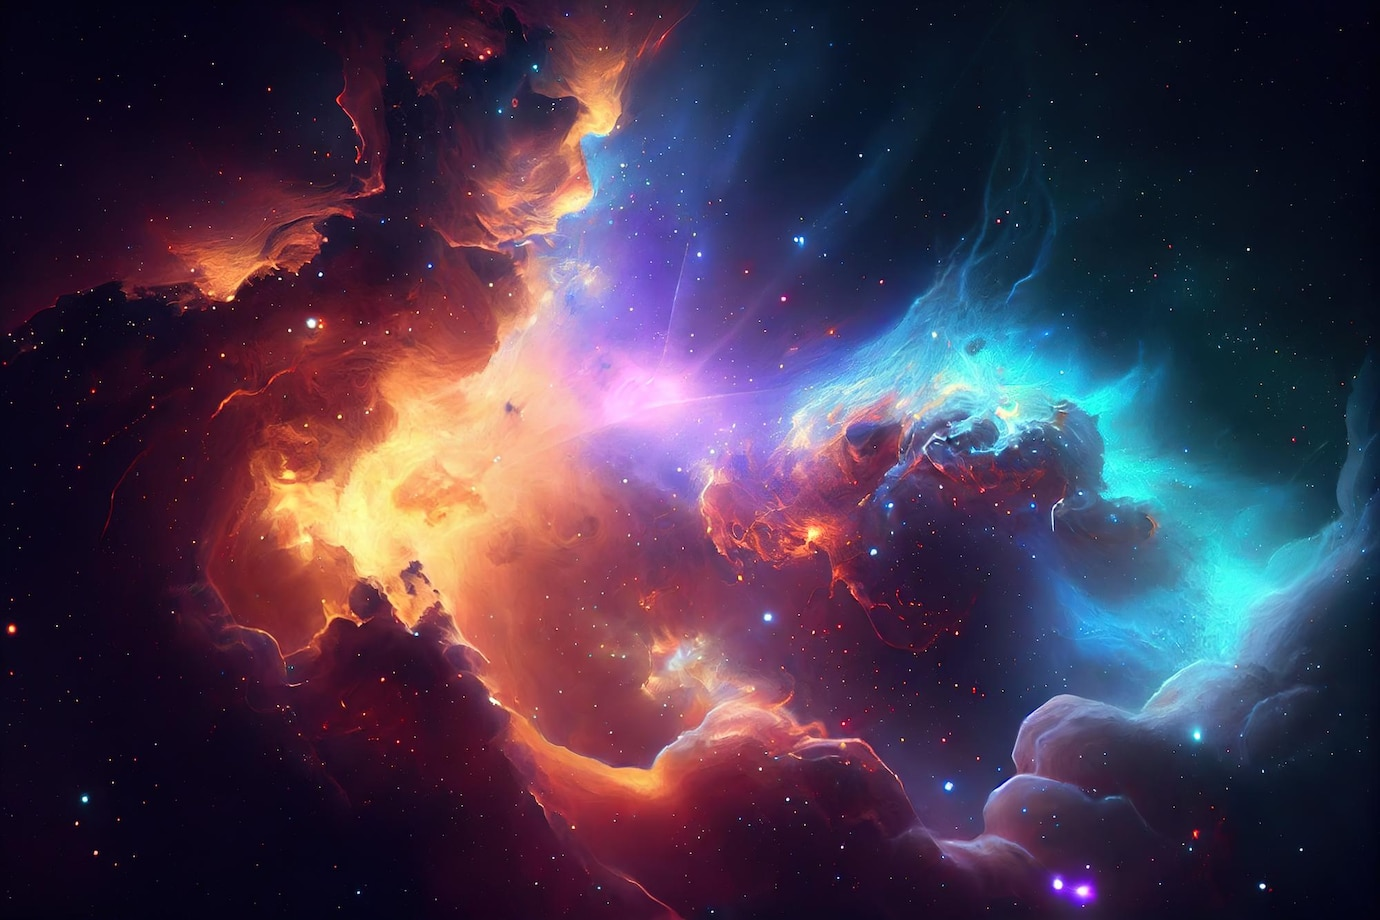
\includegraphics[width=0.5\linewidth]{galaxy}
%          \caption{View from the Webb Telescope}
%          \label{fig:galaxy1}
%  \end{figure}
 
% There's a picture of a galaxy above \ref{fig:galaxy1}.
% \end{document}

% \documentclass{article}
% \begin{document}
% \begin{itemize}
%   \item The individual entries are indicated with a black dot, a so-called bullet.
%   \item The text in the entries may be of any length.
% \end{itemize}

% \begin{enumerate}
%   \item This is the first entry in our list.
%   \item The list numbers increase with each entry we add.
% \end{enumerate}

% \end{document}

%%%%%%%%%%%%%%%%%%%%% HOW TO WRITE MATH %%%%%%%%%%%%%%%%
% \documentclass[12pt, letterpaper]{article}
% \begin{document}
% In physics, the mass-energy equivalence is stated 
% by the equation $E=mc^2$, discovered in 1905 by Albert Einstein.

% \begin{math}
% E=mc^2
% \end{math} is typeset in a paragraph using inline math mode---as is $E=mc^2$, and so too is \(E=mc^2\).


% The mass-energy equivalence is described by the famous equation
% \[ E=mc^2 \] discovered in 1905 by Albert Einstein. 

% In natural units ($c = 1$), the formula expresses the identity
% \begin{equation}
% E=m
% \end{equation}

% Subscripts in math mode are written as $a_b$ and superscripts are written as $a^b$. These can be combined and nested to write expressions such as

% \[ T^{i_1 i_2 \dots i_p}_{j_1 j_2 \dots j_q} = T(x^{i_1},\dots,x^{i_p},e_{j_1},\dots,e_{j_q}) \]
 
% We write integrals using $\int$ and fractions using $\frac{a}{b}$. Limits are placed on integrals using superscripts and subscripts:

% \[ \int_0^1 \frac{dx}{e^x} =  \frac{e-1}{e} \]

% Lower case Greek letters are written as $\omega$ $\delta$ etc. while upper case Greek letters are written as $\Omega$ $\Delta$.

% Mathematical operators are prefixed with a backslash as $\sin(\beta)$, $\cos(\alpha)$, $\log(x)$ etc.

% \end{document}

%%%%%%%%%%%%%%%%%%%%% MORE MATH %%%%%%%%%%%%%%%%

% \documentclass{article}
% \usepackage{amsmath}% For the equation* environment
% \begin{document}
% \section{First example}

% The well-known Pythagorean theorem \(x^2 + y^2 = z^2\) was proved to be invalid for other exponents, meaning the next equation has no integer solutions for \(n>2\):

% \[ x^n + y^n = z^n \]

% \section{Second example}

% This is a simple math expression \(\sqrt{x^2+1}\) inside text. 
% And this is also the same: 
% \begin{math}
% \sqrt{x^2+1}
% \end{math}
% but by using another command.

% This is a simple math expression without numbering
% \[\sqrt{x^2+1}\] 
% separated from text.

% This is also the same:
% \begin{displaymath}
% \sqrt{x^2+1}
% \end{displaymath}

% \ldots and this:
% \begin{equation*}
% \sqrt{x^2+1}
% \end{equation*}
% \end{document}

%%%%%%%%%%%%%%%%%%%%% ABSTRACT AND NEW LINES %%%%%%%%%%%%%%%%

% \documentclass[12pt]{article}
% \begin{document}
% \begin{abstract}
% This is a simple paragraph at the beginning of the 
% document. A brief introduction about the main subject.
% \end{abstract}

% After our abstract we can begin the first paragraph, then press ``enter'' twice to start the second one.

% This line will start a second paragraph.

% I will start the third paragraph and then add \\ a manual line break which causes this text to start on a new line but remains part of the same paragraph. Alternatively, I can use the \verb|\newline|\newline command to start a new line, which is also part of the same paragraph.
% \end{document}


%%%%%%%%%%%%%%%%%%%%% SECTIONS AND SUBSECTIONS %%%%%%%%%%%%%%%%

% \documentclass{book}
% \begin{document}

% \chapter{First Chapter}

% \section{Introduction}

% This is the first section.

% Lorem  ipsum  dolor  sit  amet,  consectetuer  adipiscing  
% elit. Etiam  lobortisfacilisis sem.  Nullam nec mi et 
% neque pharetra sollicitudin.  Praesent imperdietmi nec ante. 
% Donec ullamcorper, felis non sodales...

% \section{Second Section}

% Lorem ipsum dolor sit amet, consectetuer adipiscing elit.  
% Etiam lobortis facilisissem.  Nullam nec mi et neque pharetra 
% sollicitudin.  Praesent imperdiet mi necante...

% \subsection{First Subsection}
% Praesent imperdietmi nec ante. Donec ullamcorper, felis non sodales...

% \subsubsection{First Subsubsection}
% This is a nested section

% \subsubsection{Second Subsubsection}
% This is a nested section

% \section*{Unnumbered Section}
% Lorem ipsum dolor sit amet, consectetuer adipiscing elit.  
% Etiam lobortis facilisissem...

% \paragraph{First Paragraph}
% Bla bla bla paragraph

% \paragraph{Second Paragraph}
% Bla bla bla paragraph two

% \subparagraph{First Subparagraph}
% First Subparagraph

% \begin{center}
% \begin{tabular}{c c c}
%  cell1 & cell2 & cell3 \\ 
%  cell4 & cell5 & cell6 \\  
%  cell7 & cell8 & cell9    
% \end{tabular}
% \end{center}
% %%%%%%%%% VS %%%%%%%%%%
% \begin{center}
% \begin{tabular}{|c|c|c|} 
%  \hline
%  cell1 & cell2 & cell3 \\ 
%  cell4 & cell5 & cell6 \\ 
%  cell7 & cell8 & cell9 \\ 
%  \hline
% \end{tabular}
% \end{center}

% \begin{center}
%  \begin{tabular}{||c c c c||} 
%  \hline
%  Col1 & Col2 & Col2 & Col3 \\ [0.5ex] 
%  \hline\hline
%  1 & 6 & 87837 & 787 \\ 
%  \hline
%  2 & 7 & 78 & 5415 \\
%  \hline
%  3 & 545 & 778 & 7507 \\
%  \hline
%  4 & 545 & 18744 & 7560 \\
%  \hline
%  5 & 88 & 788 & 6344 \\ [1ex] 
%  \hline
% \end{tabular}
% \end{center}

% Table \ref{table:data} shows how to add a table caption and reference a table.
% \begin{table}[h!]
% \centering
% \begin{tabular}{||c c c c||} 
%  \hline
%  Col1 & Col2 & Col2 & Col3 \\ [0.5ex] 
%  \hline\hline
%  1 & 6 & 87837 & 787 \\ 
%  2 & 7 & 78 & 5415 \\
%  3 & 545 & 778 & 7507 \\
%  4 & 545 & 18744 & 7560 \\
%  5 & 88 & 788 & 6344 \\ [1ex] 
%  \hline
% \end{tabular}
% \caption{Table to test captions and labels.}
% \label{table:data}
% \end{table}

% \end{document}

%%%%%%%%%%%%%% TABLE OF CONTENTS %%%%%%%%%%%

\documentclass{article}
\title{Sections and Chapters}
\author{Ibrahim Khalilov}
\date{January 2024}
\begin{document}
  
\maketitle % Make the above a title
  
\tableofcontents

\section{Introduction}
   
This is the first section.
      
Lorem  ipsum  dolor  sit  amet,  consectetuer  adipiscing  
elit.   Etiam  lobortisfacilisis sem.  Nullam nec mi et 
neque pharetra sollicitudin.  Praesent imperdietmi nec ante. 
Donec ullamcorper, felis non sodales...
       
\section*{Unnumbered Section}
\addcontentsline{toc}{section}{Unnumbered Section}

Lorem ipsum dolor sit amet, consectetuer adipiscing elit.  
Etiam lobortis facilisissem.  Nullam nec mi et neque pharetra 
sollicitudin.  Praesent imperdiet mi necante...

\section{Second Section}
       
Lorem ipsum dolor sit amet, consectetuer adipiscing elit.  
Etiam lobortis facilisissem.  Nullam nec mi et neque pharetra 
sollicitudin.  Praesent imperdiet mi necante...
\end{document}

